\documentclass{article}
\usepackage{tikz}

\begin{document}

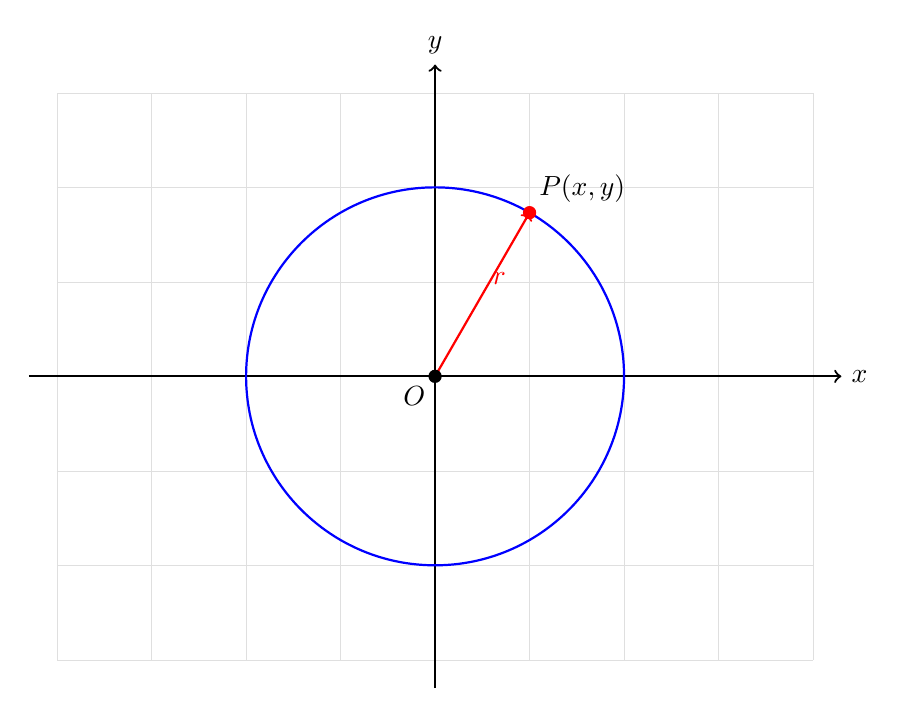
\begin{tikzpicture}[scale=1.2]

    % Grid
    \draw[step=1cm, gray!25, very thin] (-4,-3) grid (4,3);

    % Axes
    \draw[->, thick] (-4.3,0) -- (4.3,0) node[right] {$x$};
    \draw[->, thick] (0,-3.3) -- (0,3.3) node[above] {$y$};

    % Circle
    \draw[thick, blue] (0,0) circle (2);

    % Radius
    \draw[->, thick, red] (0,0) -- (60:2)
        node[midway, above right] {$r$};

    % Point
    \fill[red] (60:2) circle (2pt);
    \node[above right] at (60:2) {$P(x,y)$};

    % Origin
    \fill (0,0) circle (2pt);
    \node[below left] at (0,0) {$O$};

\end{tikzpicture}

\end{document}
